\chapter{Processi e metodologie}
\label{cap:processi-metodologie}

\intro{Brevissima introduzione al capitolo}\\

\section{Material Design}
% Nome, riscrittura senza ripetizioni del contesto (presentazione simil "marketing")
%L'applicazione è stata creata seguendo la regole di Material Design di Goggle  e i consigli di Material Components messi a disposizione da Flutter (https://docs.flutter.dev/ui/widgets/material).\newline
%Per permettere la navigazione tra le varie pagine dellàapplicazione, è stato utilizzato una barra di navigazione posta sulla lato inferiore della schermata (Figura ???)
Alla base dell'applicazione, è stato scelgo di seguire il Material Design (Figura \ref{fig:material}) (https://m3.material.io/) sviluppato da Google, che si concentra su un maggiore uso di layout basati su una griglia, animazioni, transizioni ed effetti di profondità come l'illuminazione e le ombre.\newline
Si tratta di una serie di regole ideate per consentire una buona UX (User Expirence) e definire una UI (User Interface) per l'utente da implementarre in ambiente Web, Android e in Flutter.\newline
Viene annunciato per la prima volta da Google il 25 giugno del 2014 durante il Google I/O, una conferenza organizzata annualmente da Google a Mountain View, in California.\newline
Venne rinnovato nel 2018 con il Material Design 2, anche chiamato Google Material Theme, introducendo un maggiore utilizzo di angoli arrotondati, spazi bianchi e icone colorate, infine viene rinnovato nel 2021 con il Material Design 3, oppure Material You, introducendo l'uso di tasti più grandi e maggiore uso delle animazioni.\newline
Oggi viene ancora utilizzato il Material Design 3 ed è stato seguito per lo sviluppo dell'app dei pranzi.\newline
Per consentire l'uso dei propri prodotti software a più utenti possibili, il Material Design segue le regole del WCAG (Web Content Accessibility Guidelines) (https://www.w3.org/WAI/standards-guidelines/wcag/), mettendo alla base di ogni progetto l'accessibilità, creando così dei prodotti inclusivi, cioè usabili anche da chi ha delle disabilità e deve utilizzare dei software o dei tool appositi, come per esempio un lettore di testo.\newline
I layout devono essere studiati in modo da guidare l'utente nella navigazione della pagina e devono essere dinamici, in modo che le pagine si addattino ad ogni tipo di schermo.\newline
Vengono indicate delle regole precise su come devono essere impostate le componenti, come devono essere raggrupente, lo spazio che deve esserci e tanti altri piccoli ma importanti dettagli che lo sviluppatore deve considerare per permettere all'utente di orientarsi su qualsiasi dispositivo.\newline
Anche Flutter offre una guida sulle componenti che mette a disposizione per lo sviluppatore e che sono state ideate per rispettare le regole di Material Design appena descritte (https://docs.flutter.dev/ui/widgets/material).\newline
\begin{figure}[!h] 
    \centering 
    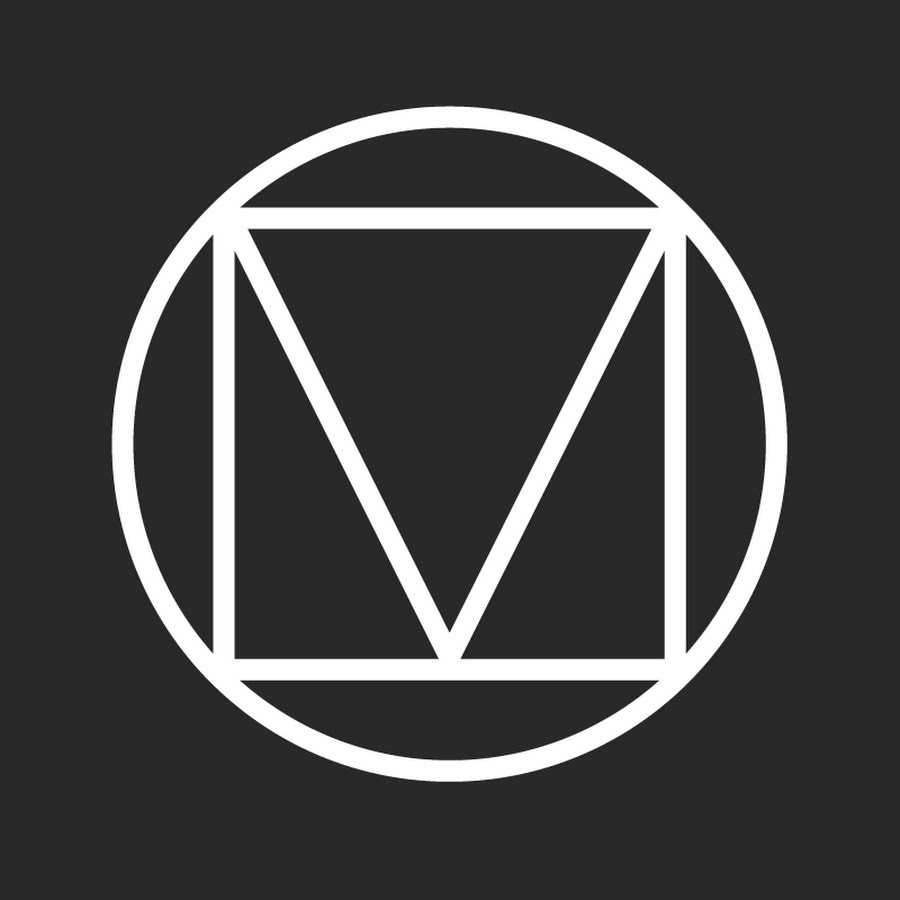
\includegraphics[width=0.2\columnwidth]{MaterialDesign} 
    \caption{Logo del Material Design di Google}\label{fig:material}
\end{figure}

\section{Processi di sviluppo}
%Ho lavorato con Sprint in Agile o altro...

\section{Tecnologie}

\subsection{Flutter}
Flutter (Figura \ref{fig:flutter}) è un progetto open-source di Google il cui vantaggio principale è la generazione di applicazioni multipiattaforma a partire da un unico codice sorgente.\newline
Permette quindi allo sviluppatore di concentrarsi sul prodotto da realizzare senza dover preferire un sistema operativo mobile ad un altro.\newline
Per questo motivo è stato scelto di utilizzare Flutter come framework principale, dato che il prodotto finale deve funzionare sia per dispositivi Android sia per dispositivi iOS.\newline
%\begin{figure}[!h] 
%    \centering 
%    
\includegraphics[width=0.45\columnwidth]{Flutter} 
%    \caption{Logo di Flutter}\label{fig:flutter}
%\end{figure}

\subsection{Dart}
Il linguaggio sul quale si basa Flutter è Dart (Figura \ref{fig:dart}), il quale nacque con l’intento di sostituire JavaScript come protagonista delle applicazioni web.\newline
Tra i suoi pregi si elencano il compilatore JIT, migliore gestione della sicurezza, la velocità e la maggiore scalabilità.\newline
Il paradigma principale è l’orientamento agli oggetti, una sua particolarità è data dalla sua attenzione alla null safety per la quale nessun valore può essere nullo a meno che questa possibilità non sia esplicitamente dichiarata.\newline
%\begin{figure}[!h] 
%    \centering 
%    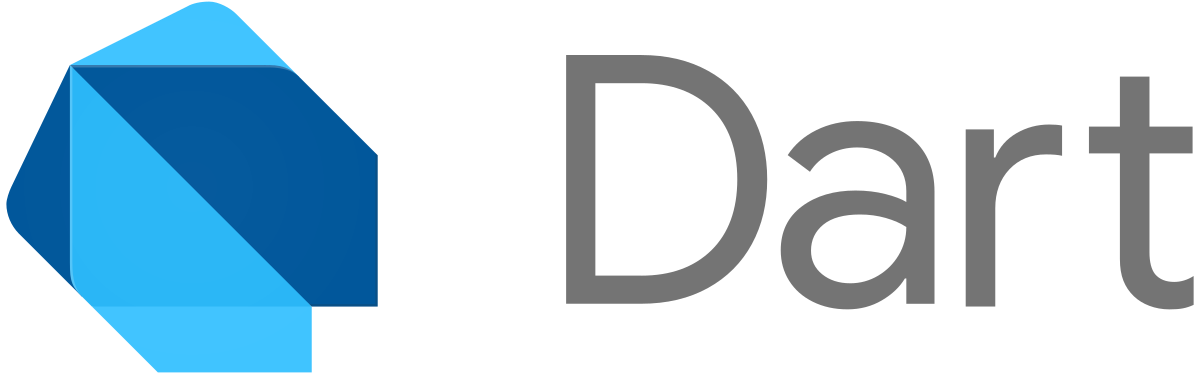
\includegraphics[width=0.4\columnwidth]{Dart} 
%    \caption{Logo di Dart}\label{fig:dart}
%\end{figure}

\subsection{Firebase}
Firebase (Figura \ref{fig:dart}) è una piattaforma open-source per la creazione di applicazioni per dispositivi mobili e web sviluppata da Google.\newline
Firebase sfrutta l'infrastruttura di Google e il suo cloud per fornire una suite di strumenti per scrivere, analizzare e mantenere applicazioni cross-platform.\newline
Infatti offre funzionalità come analisi, database (usando strutture noSQL), messaggistica e segnalazione di arresti anomali per la gestione di applicazioni web, iOS e Android.\newline
Per lo sviluppo dell'app sono stati utilizzati:
\begin{itemize}
    \item Firebase Autenticathion, per permettere la registrazione e l'autenticazione di un utente tramite mail e password
    \item Cloud Firestore, per la gestione del database.
\end{itemize}
%\begin{figure}[!h] 
%    \centering 
%    
\includegraphics[width=0.55\columnwidth]{Firebase} 
%    \caption{Logo di Firebase}\label{fig:figma}
%\end{figure}

\subsection{Figma}
Figma (Figura \ref{fig:figma}) è un software per la progettazione di User Interface(UI).\newline
Permette infatti di realizzare prototipi delle interfacce, altresì detti mockup, che permettono di illustrare il risultato finale che si desidera ottenere.\newline
Questo strumento è stato utilizzato per mostrare e concordare l'interfaccia dell'app al tutor aziendale, prima della fase di codifica.\newline
%\begin{figure}[!h] 
%    \centering 
%    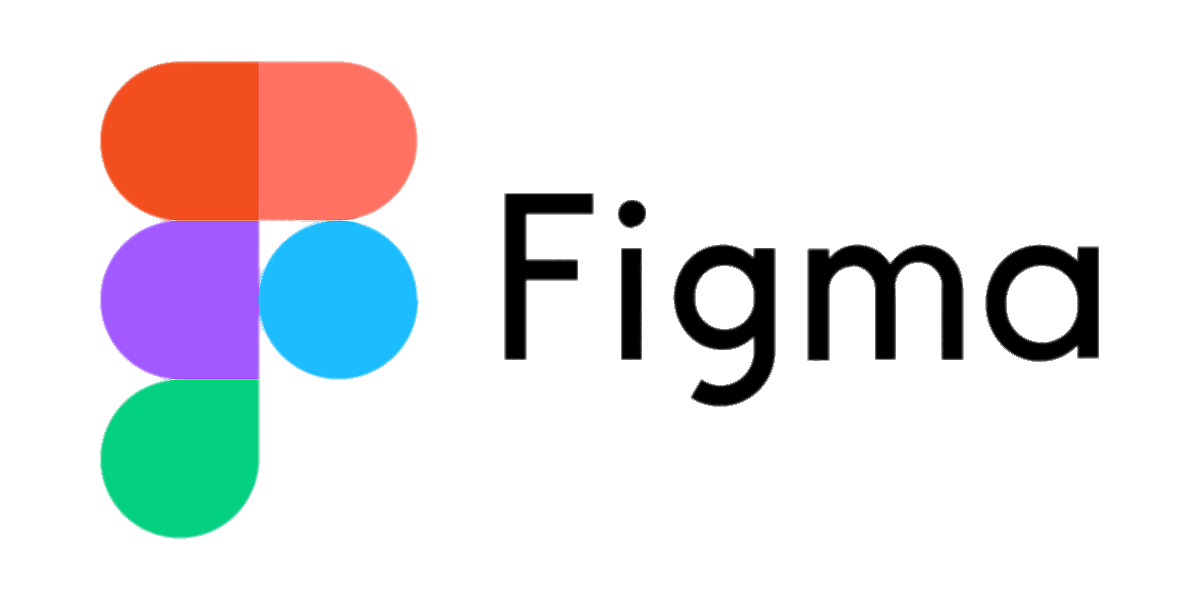
\includegraphics[width=0.38\columnwidth]{Figma} 
%    \caption{Logo di Figma}\label{fig:figma}
%\end{figure}



\subsection{Android Studio}
Android Studio (Figura \ref{fig:android}) è un ambiente di sviluppo integrato adibito per la creazione di applicazioni Android e mette a disposizione dei simulatori virtuali di uno o più cellulari con sistema operativo Android.\newline
Il progetto è stato sviluppato interamente con l'uso di questo IDE ed è stato utilizzato il simulatore virtuale di Google Pixel 7 con sistema operativo Android 13 per testare la build dell'app.\newline
%\begin{figure}[!h] 
%    \centering 
%    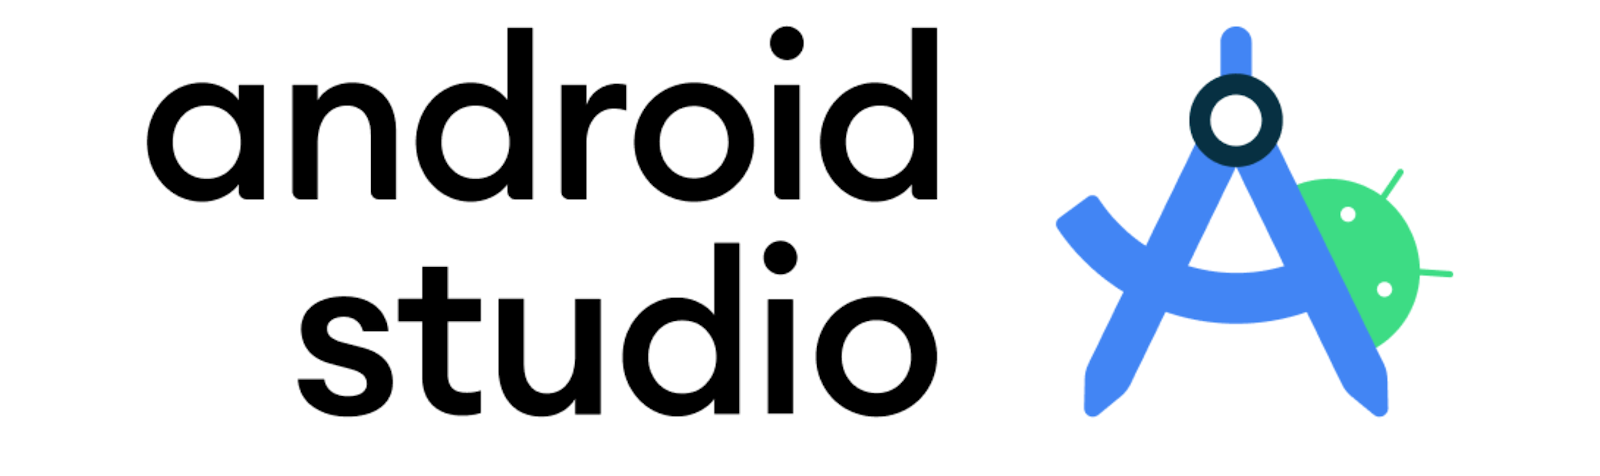
\includegraphics[width=0.5\columnwidth]{AndroidStudio} 
%    \caption{Logo di Android Studio}\label{fig:android}
%\end{figure}

\subsection{Xcode}
Xcode (Figura \ref{fig:apple}) è un ambiente di sviluppo integrato (Integrated development environment, IDE), completamente sviluppato e mantenuto da Apple, contenente una suite di strumenti utili allo sviluppo di software per i sistemi macOS, iOS, iPadOS, watchOS e tvOS.\newline
Per poter testare la build del progetto, è stato utilizzato il simulatore virtuale di iPhone 15 con sistema operativo iOS 17, messo a disposizione da questo software.\newline
%\begin{figure}[!h] 
%    \centering 
%    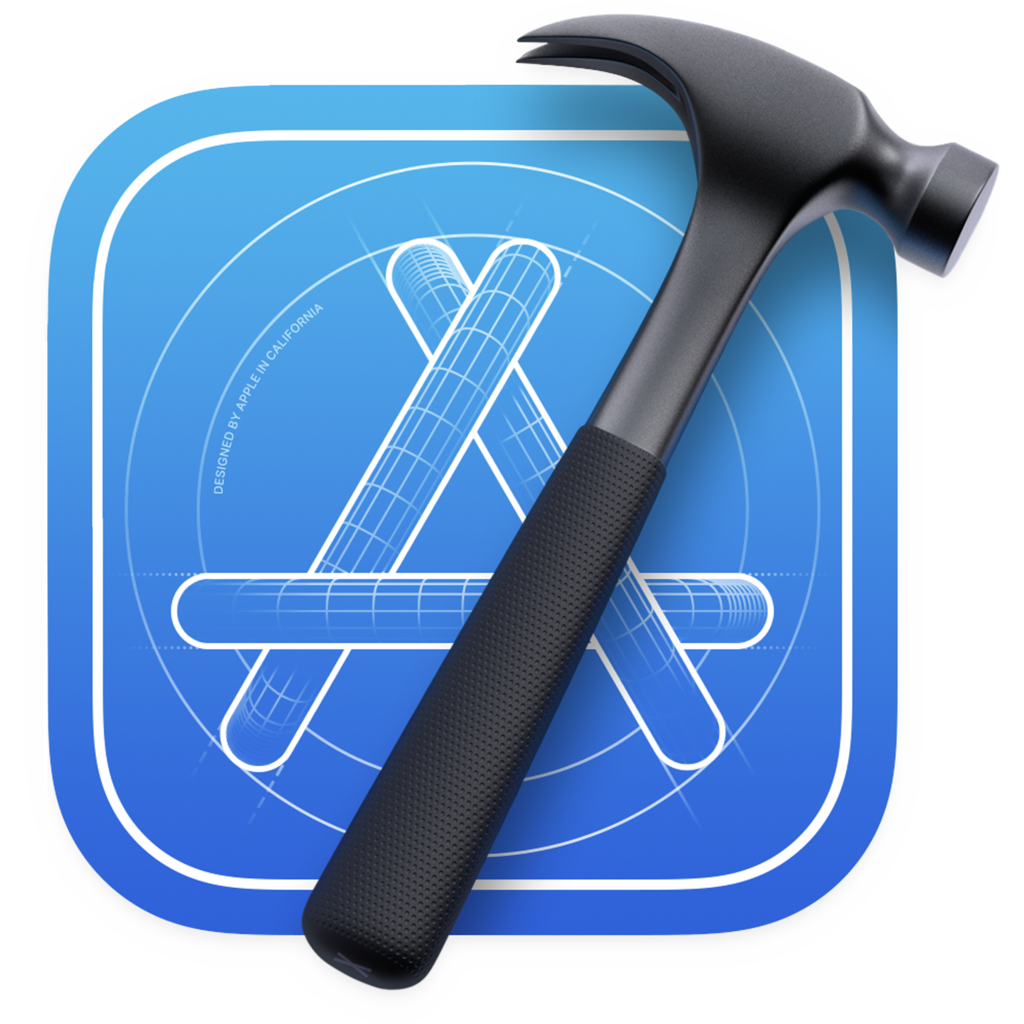
\includegraphics[width=0.4\columnwidth]{Xcode} 
%    \caption{Logo di Android Studio}\label{fig:apple}
%\end{figure}

\subsection{GitHub}
GitHub (Figura \ref{fig:github}) è una piattaforma di hosting per repository git.\newline
Fornisce agli sviluppatori strumenti per migliorare e mantenere il codice come:
\begin{itemize}
    \item features utilizzabili da linea di comando,
    \item gestione delle pull request e code review,
    \item strumenti per l’issue tracking.
\end{itemize}
La codebase della piattaforma RiskApp è suddivisa in varie repository su GitHub.\newline
Per questo progetto, l'azienda ha riservato una repository apposta per permettermi di lavorare in autonomia al codice.\newline
%\begin{figure}[!h] 
%    \centering 
%    
\includegraphics[width=0.5\columnwidth]{GitHub} 
%    \caption{Logo di GitHub}\label{fig:github}
%\end{figure}

\subsection{Slack}
Slack (Figura \ref{fig:slack}) è un applicazione multipiattaforma per la messaggistica istantanea tra membri di un gruppo di lavoro.\newline
Una delle funzioni di Slack è la possibilità di organizzare la comunicazione del team attraverso canali specifici, canali che possono essere accessibili a tutto il team o solo ad alcuni membri.\newline
È possibile inoltre comunicare con il team anche attraverso chat individuali private o chat con due o più membri.\newline
Questo software è stato utilizzato per comunicare con il tutor aziendale da remoto e per condividere materiale.\newline
%\begin{figure}[!h] 
%    \centering 
%    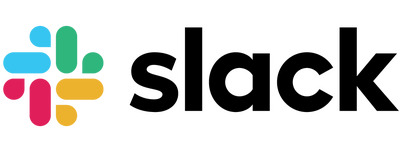
\includegraphics[width=0.4\columnwidth]{Slack} 
%    \caption{Logo di Slack}\label{fig:slack}
%\end{figure}
